%!TEX root = thesis.tex
\chapter{Evolution of Thermal Flux in Asymmetric Thin-Films}
\label{chap:diff_boundary}
\section{Introduction}\blfootnote{Portions of this chapter have originally been published in \cite{ownSpatialTF} ``Spatial Manipulation of Thermal Flux in Nanoscale Films" (2017), \textit{Nanoscale and Microscale Thermophysical Engineering}, Vol. 21 (3), published by Taylor \& Francis.} 
 Although studies on the reduction in thermal conductivity of nanoscale thin films have attracted significant interest in recent years \cite{RN286,RN120,RN46,RN127,RN207,RN204,maldovan2011tf,RN189,RN208}, the spatial distribution of the heat flux and the possibility of modulating the flow of thermal energy within the nanostructure have received little attention. In this chapter, we study the effect of distinct surface properties on thermal transport in asymmetric thin-films. Previously in \Cref{chap:predictive}, we showed the development of thermal transport model for thin-films that assumed that the thin-film was symmetric, i.e. both the boundaries possessed identical surface features. Here, we extend the previous model to move beyond the symmetric nanostructure approximation and use the developed model to study the role of film thickness, alloying, and temperature on spatial distribution of thermal flux within thin films. We show that designing the physical properties of thin-film surfaces provides a control over the path taken by the thermal energy; for example, whether heat flows close to a surface or near the center of the film. We also show the strong dependence of these spatial flux profiles on the film thickness, temperature and alloying. The results presented in this work are valuable for the interpretation of theoretical and experimental measurements of thermal conductivities in semiconductor thin films, especially in the general case where the two surfaces of thin films may possess distinct surface specularities independent of one another, for which currently there are no theoretical models that can connect computations with measurements. Our findings help to advance the understanding of the nature of thermal fluxes within reduced geometries and provide an avenue for better integration of experimental and computational research efforts in the area of nanoscale thermal transport.
\section{Methodology}\label{sec:ch3-method}
The failure of Fourier’s laws at small length and timescales in nanoscale thin films marks a shift away from fully diffusive transport to a quasi-ballistic regime and necessitates the treatment of heat conduction via phonon transport. In the kinetic picture of quasi-ballistic transport, since the mean-free-paths of heat conducting phonons are longer than the thickness of the thin-films, it causes a change in their ability to conduct heat. In the phononic populations approach, this change in thermal properties can be understood as the deviation of phonon populations away from equilibrium. Here, we show \textit{two equivalent methodologies} that approach this transport physics in thin-films from the kinetic picture and phononic population perspective, respectively. 	
\subsection{System Description}
The system of interest is a thin-film [\Cref{fig:ch3-schematic}, top], of thickness \gls{t}. The surfaces of the thin-film are assumed to be independent of each other, thus have distinct surface properties in general. These distinct surface properties give rise to their individual specularity parameters, denoted as $p^{L}$ and $p^{U}$ for the lower and upper surface, respectively. Importantly, in both the formulations the surface specularity \gls{p} is not an arbitrary parameter but rather describes the physical interactions between phonons and thin-film boundaries and depends on the surface characteristics (roughness and correlation length) and phonon properties (incident angle on the surface and momentum), and physically represents the proportion of phonons that are specularly scattered upon interacting with the surface.

% schematic
\begin{figure}[hbt]
	\centering 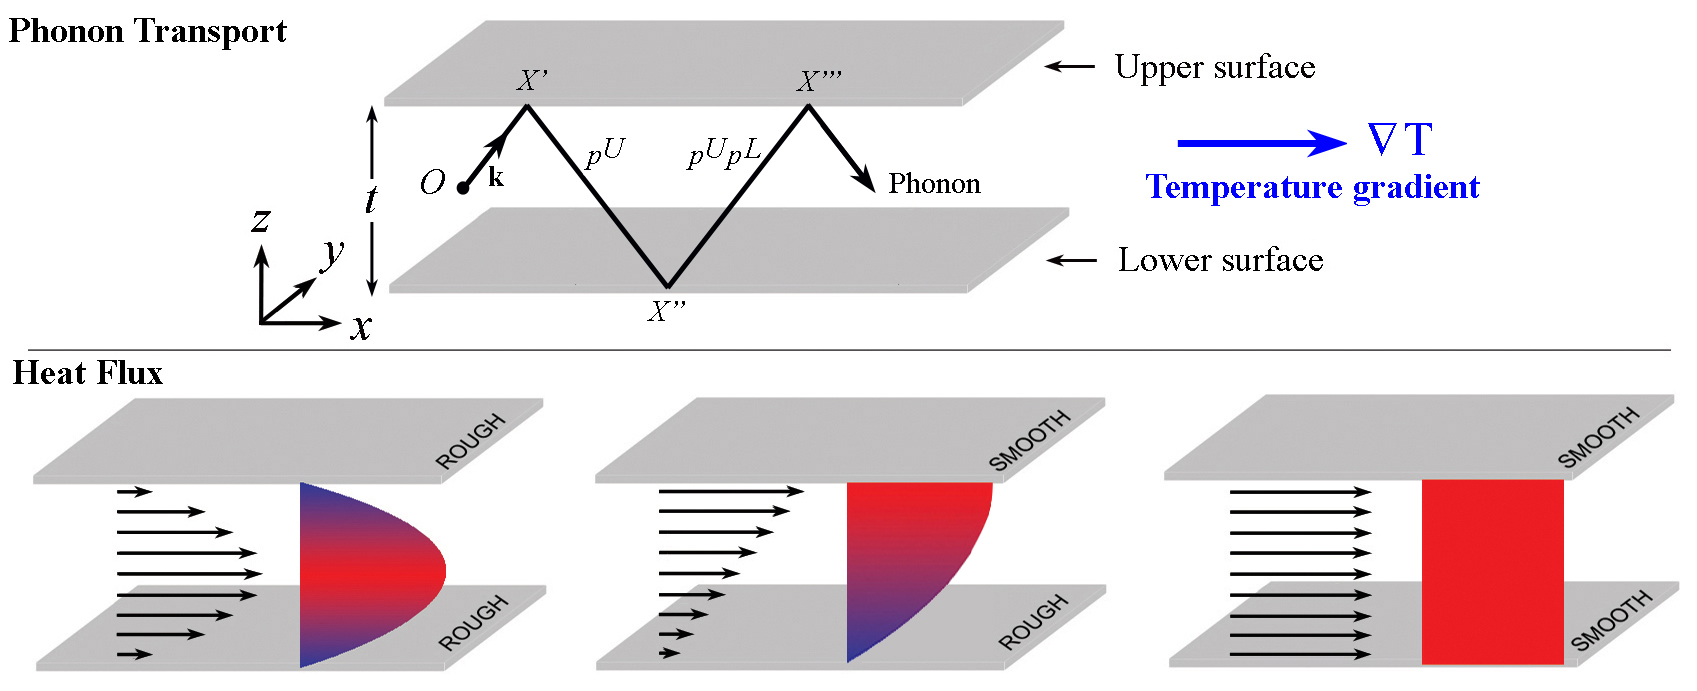
\includegraphics[width=\textwidth]{/ch3/Fig1.jpg}
	\caption{Top: Schematic representation of phonon transport in thin films where phonons originating at point O inside a thin film of thickness \gls{t} move under a thermal gradient \gls{gradT} along the in-plane direction. In the figure, the wavevector \gls{k} leads the phonon toward the upper surface possessing surface specularity $p^{U}$ and upon scattering is directed toward the lower surface possessing surface specularity $p^{L}$. Bottom: Schematic representation of heat flux spatial distribution within thin films depending on the surface conditions (smooth or rough) of the boundaries.}
	\label{fig:ch3-schematic}
\end{figure}

\subsection{Reduced Mean-Free-Path Approach}
Similar to the derivation shown in \Cref{sec:MFPRedModel}, we evaluate the changes in phononic mean-free-paths \gls{mfp}. Here, however, since the two surfaces are distinct, the model needs to differentiate among phonons originating with positive and negative wave vectors along the z-coordinate [\Cref{fig:ch3-schematic}, top]. For example, phonons with positive $\mathbf{k}_{z}$ will see first the upper surface at $z = t$ and will thus be first scattered at point $X^{'}$ accompanied by change in sign of $\vec{k}_{z}$. At every interaction with the upper surface, a proportion of phonons, $1-p^{U}$ are scattered diffusively. Similarly, phonons with initial negative $\mathbf{k}_{z}$ interact with lower surface at $z=0$ first where $1-p^{L}$ proportion of incident phonons are scattered diffusively. By writing $OX^{'}=\Lambda$, the contribution to the mean-free-path for phonons up to the point $X^{'}$ is evaluated to be,

\begin{equation}
\ell_{\vec{k}}^{{OX^{'}}}=\int_{0}^{\Lambda}{\frac{r}{\ell_{\vec{k}}^{\textrm{bulk}}}\exp\Big({-\frac{r}{\ell_{\vec{k}}^{\textrm{bulk}}}} \Big)\,dr} + (1-p^{U})\int_{\Lambda}^{\infty} {\frac{\Lambda}{\ell_{\vec{k}}^{\textrm{bulk}}}\exp\Big({-\frac{r}{\ell_{\vec{k}}^{\textrm{bulk}}}}\Big)\,dr}
\label{eq:ox}
\end{equation} 
For phonons subsequently specularly reflected and moving between $X^{'}$ and $X^{''}$, the contribution to the mean-free-path can analogously be written as,
\begin{equation}
\ell_{\vec{k}}^{{X^{'}X^{''}}}=p^{U}\int_{\Lambda}^{\Lambda+\Lambda^{*}}{\frac{r}{\ell_{\vec{k}}^{\textrm{bulk}}}\exp\Big({-\frac{r}{\ell_{\vec{k}}^{\textrm{bulk}}}} \Big)\,dr} + p^{U}(1-p^{L})\int_{\Lambda+\Lambda^{*}}^{\infty} {\frac{\Lambda+\Lambda^{*}}{\ell_{\vec{k}}^{\textrm{bulk}}}\exp\Big({-\frac{r}{\ell_{\vec{k}}^{\textrm{bulk}}}}\Big)\,dr}
\label{eq:xx}
\end{equation} 
Note that the first term in \Cref{eq:xx} represents the contribution of the fraction $p^{U}$ of phonons that are specularly reflected at $X^{'}$ and the second term represents the contribution of the fraction $p^{U} (1-p^{L})$ of phonons that are diffusively scattered upon interacting with the surface at $X^{''}$. The total reduced mean-free-path can be obtained by summing the contributions from terms in \Cref{eq:ox,eq:xx} and the successive terms expanded similarly, which yields the general form of the reduced mean-free-path for a thin film with arbitrary, distinct surface specularities at the film boundaries as:

\begin{equation}
\ell_{\vec{k}}(z)= 
\begin{cases}
\ell_{\vec{k}}^{\textrm{bulk}}\Bigg(\dfrac{1-\Theta_1 + p^L p^U \Theta_2 \Theta_3 - (1-p^U + p^U \Theta_2 ) \Theta_3 }{1-\Theta_1}\Bigg) & \text{if}\: \vec{k}_z >0 \\
\ell_{\vec{k}}^{\textrm{bulk}}\Bigg(\dfrac{1-\Theta_1 + p^L p^U \Theta_2 \Theta_3 - (1-p^L + p^L \Theta_2 ) \Theta_3 }{1-\Theta_1}\Bigg) & \text{if}\: \vec{k}_z <0	
\end{cases}
\label{eq:mfp_ch3}
\end{equation} 
where,
\begin{align}\label{eq:mfp_params_ch3}
	\Theta_1 &= p^L p^U \exp (-2\Lambda^*/\ell_{\vec{k}}^{\textrm{bulk}}) \nonumber \\
	\Theta_2 &= \exp (-\Lambda^*/\ell_{\vec{k}}^{\textrm{bulk}}) \\
	\Theta_3 &= \exp (-\Lambda/\ell_{\vec{k}}^{\textrm{bulk}}) \nonumber
\end{align}

Thus, \Cref{eq:mfp_ch3,eq:mfp_params_ch3} are used to obtain the reduced phonon mean-free-paths which depend on the spatial position within the thin-film. Thus, the thermal flux obtained using these mean-free-paths is dependent on the spatial position as indicated by the integrand of the spatial domain in \Cref{eq:phonon_fourier}. 

\subsection{Non-equilibrium Population Distribution Approach}
The local population of phonons \gls{f}$(r)$ in a thin-film under an in-plane gradient is deviated from equilibrium Bose-Einstein distribution \gls{fBE}. For a steady state BTE (see \Cref{eq:bte_ss}) applied to a thin-film, the solution to non-equilibrium phonon populations can be written as \cite{book_Ziman}:

\begin{equation}\label{eq:ch3-5}
  f_\vec{k}=  f_\vec{k}^{BE}-\tau_\vec{k}\frac{\partial f_\vec{k}^{BE}}{\partial T}\Bigg(1+\Phi_\vec{k}\exp\Big(-\dfrac{z}{\tau_\vec{k} v_\vec{k}}\Big)\Bigg)v_\vec{k}\cdot \nabla T 
\end{equation}
where $\Phi_\vec{k}$ is determined by the boundary conditions of the thin-film. As a result, a closed-form solution of the BTE in terms of local phonon populations or equivalently, in terms of a deviation function $g_\vec{k} = f_\vec{k} - f_\vec{k}^{BE}$ of phonon populations from equilibrium, can be obtained by imposing the boundary conditions for the thin-film geometry. The boundary conditions can be written following a balance of phonon populations incoming and outgoing from the surfaces. The phononic deviation functions are divided into two components, $g_\vec{k}^+$ and $g_\vec{k}^-$ denoting the populations with positive and negative z-components of \gls{k}.
\begin{align}\label{eq:boundary_conditions_ch3_1}
	[f^{BE}+g_\vec{k}^+(z=0)] &= p^L [f^{BE}+g_\vec{k}^-(z=0)]+[1-p^L]f^{BE} \\
	[f^{BE}+g_\vec{k}^-(z=t)] &= p^U [f^{BE}+g_\vec{k}^+(z=t)]+[1-p^U]f^{BE}
\label{eq:boundary_conditions_ch3_2}
\end{align}

Using \Cref{eq:boundary_conditions_ch3_1,eq:boundary_conditions_ch3_2}, the deviation from equilibrium can be calculated to be,
\begin{equation}\label{eq:ch3_g}
g_\vec{k}(z)=
\begin{cases} 
-\tau_\vec{k}v_{\vec{k}|x}\frac{\partial f_\vec{k}^{BE}}{\partial T}\frac{\partial T}{\partial x}\Big[1-\frac{1-p^L+p^L(1-p^U)\exp(-t/\tau_\vec{k}v_{\vec{k}|z})}{1-p^Lp^U\exp(-2t/\tau_\vec{k}v_{\vec{k}|z})}\exp\Big(-\dfrac{z}{\tau_\vec{k}v_{\vec{k}|z}}\Big) \Big] & \: \vec{k}_z >0 \\
-\tau_\vec{k}v_{\vec{k}|x}\frac{\partial f_\vec{k}^{BE}}{\partial T}\frac{\partial T}{\partial x}\Big[1-\frac{1-p^U+p^U(1-p^L)\exp(t/\tau_\vec{k}v_{\vec{k}|z})}{1-p^Lp^U\exp(2t/\tau_\vec{k}v_{\vec{k}|z})}\exp\Big(-\dfrac{z-t}{\tau_\vec{k}v_{\vec{k}|z}}\Big) \Big] & \: \vec{k}_z <0
% & \: \vec{k}_z <0	
\end{cases}
\end{equation}
where the $x$ and $z$ in the subscripts represent the components along those Cartesian directions. 
\subsection{Equivalence of Approaches}
In order to establish the fundamental equivalence of the two mathematical interpretations of behavior of phonons i.e. the kinetic approach to model modified phononic mean-free-paths and the deviation of phononic populations from equilibrium, we calculate the spatially averaged thermal conductivity from the two approaches using \Cref{eq:phonon_fourier} and \Cref{eq:pop_fourier}, respectively. We create test cases covering a range of conditions under varying roughness, correlation lengths, temperature and thin-film thickness which are detailed in \Cref{tab:parameters-validation}. 
\\
% This is a table
\begin{table}[hbt]
\centering
\caption{Test cases to examine the equivalence between reduced mean-free-path approach and deviation of population from equilibrium approach.}
\resizebox{\linewidth}{!}{%
\begin{tabular}{lcccccc} 
\toprule[\heavyrulewidth]\toprule[\heavyrulewidth]
Case \# & Thickness~(nm) & \begin{tabular}[c]{@{}l@{}}Upper Surface \\Roughness (nm)\end{tabular} & \begin{tabular}[c]{@{}l@{}}Lower Surface \\Roughness (nm)\end{tabular} & $\mathcal{L}^U/\eta^U$ & $\mathcal{L}^L/\eta^L$ & Temperature (K)  \\ 
\hline
A       & 30             & 0.5                                                                    & 0.5                                                                    & 8              & 10             & 300             \\
B       & 50             & 0.1                                                                    & 0.5                                                                    & 10             & 8              & 50              \\
C       & 100            & 0.5                                                                    & 0.5                                                                    & 10             & 10             & 300             \\
D       & 200            & 0.01                                                                   & 1.0                                                                    & 20             & 6              & 800             \\
E       & 500            & 0.25                                                                   & 1.5                                                                    & 15             & 8              & 300             \\
F       & 2000           & 0.5                                                                    & 0.5                                                                    & 10             & 10             & 300             \\
\bottomrule[\heavyrulewidth]
\end{tabular}
}
\label{tab:parameters-validation}
\end{table}

Average conductivity is evaluated using the gradient along with the integral of local flux distributions over the thickness of the film. The comparison of the conductivities is presented in \Cref{fig:ch3-validation}, from which it is evident that the two approaches generate nearly identical values of thermal conductivities for different values of thickness and surface properties which establishes the equivalency between the methods. The adjusted R-square of the linear fit between calculated values from the two approaches for the six cases is \textgreater 0.999, establishing the equivalence. Since the two approaches are mathematically equivalent, further analysis can be conducted by proceeding with any of the two methods without any loss of generality. In \Cref{sec:results_ch3}, we choose to use the reduced mean-free-path approach to calculate transport properties for two major reasons. Firstly, reduced mean-free-path approach preserves the mean-free-paths of phonons explicitly which are an important physical quantity especially for rational design of materials and in understanding behavior of phonons and heat at nanoscale. Secondly, a higher computational efficiency is achieved in the numerical integration routine in reduced mean-free-path approach reducing the cost of implementation.
% schematic
\begin{figure}[hbt]
	\centering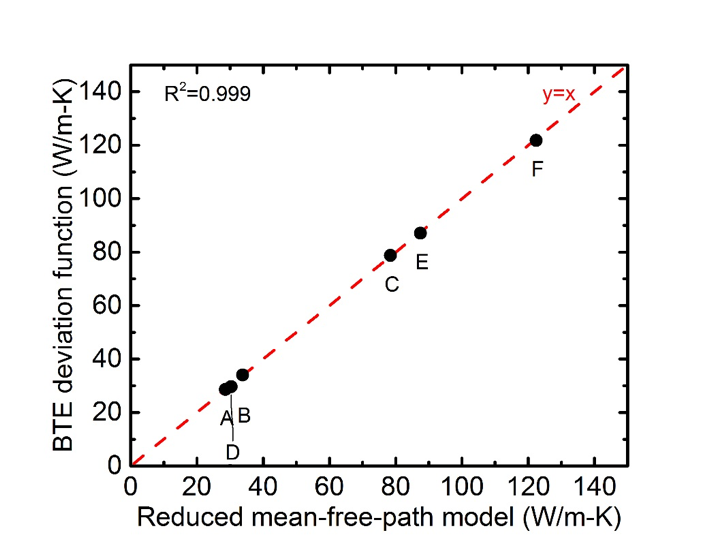
\includegraphics[width=0.75\textwidth]{/ch3/Fig2.png}
	\caption{Comparison between averaged thermal conductivity obtained from reduced mean-free-path model ($x$-axis) and deviation function via a semi-analytical BTE solution ($y$-axis), showing the equivalence of the two approaches}
	\label{fig:ch3-validation}
\end{figure}

\subsection{Note on Surface Specularity}
To obtain the surface specularity at the distinct thin-film boundaries, we utilize our previously developed (see \Cref{sec:BK}) BK surface scattering model extended with surface shadowing effects on heat conduction. The surface specularity \gls{p} obtained from the BK and shadowing theory contains a description of phonon–surface scattering that accounts for its dependence on all relevant physical variables -- phonon properties (momentum and incident angle \gls{thetai} via the wave-vector \gls{k}) and surface characteristics (roughness \gls{eta} and correlation length \gls{cl}); that is, $p = p(k, \theta_i, \eta, \mathcal{L})$.

\section{Results and Discussion}\label{sec:results_ch3}
Using our approach, we move beyond simplifying assumptions about phonon-surface scattering (e.g., constant specularity or complete diffuse scattering) in thin films and connect the physical properties of general surfaces with the spatial distribution of the thermal flux within the thin films. We note that the analogy between transport of momentum, heat, and mass has been central in many fields of engineering \cite{book_Bird}. For continuum fluids, the “no-slip” condition at a solid-fluid interface generates fluid flux spatial distributions in a number of interesting fluid phenomena, including the dynamics of falling films, flow in confined geometries, and boundary layers. Interestingly, such no-slip behavior of momentum-flux has no classical analogue in thermal transport at the continuum bulk scale. However, the existence of spatial boundaries in thin films creates a thermal flux that is a function of the spatial location within the film, analogous to fluid dynamics. 

Before analyzing the effects of surface conditions on local heat flux distributions, we apply our methodology to a particular case of a thin film of thickness \gls{t} = 100 nm at room temperature under a temperature gradient (1 K/\si{\micro}m) with equal surface properties on the two very rough boundaries (i.e., complete diffusive scattering). \Cref{fig:ch3-comparison} shows the effect of phonon–surface interactions on the local heat flux and quantitatively shows that heat conduction in a thin film with completely diffusive boundaries can be considered analogous to no-slip fluid flow in a rectangular pipe with fixed walls in the sense that the thermal flux reaches a maximum at the center. However, a clear distinction between momentum and heat transport in the form of a nonzero local value of heat flux near diffusive domain boundaries should be noted. The physical mechanism behind this spatial dependence of thermal flux distribution is the momentum randomization of diffusively scattered phonons at the surfaces, which reduces the phonon mean-free-paths depending on the distance between the surface and the point where the phonon originates [\Cref{fig:ch3-schematic}]. The agreement in the values of normalized flux for the particular case of identical diffusive surfaces \cite{RN445,RN276} serves as validation of the reduced mean-free-path methodology. Our proposed model, however, allows us to consider more general and realistic surface conditions, including different surface roughnesses and correlation lengths, as well as independent surface conditions on the two boundaries of the films.
%figure
\begin{figure}[hbt]
	\centering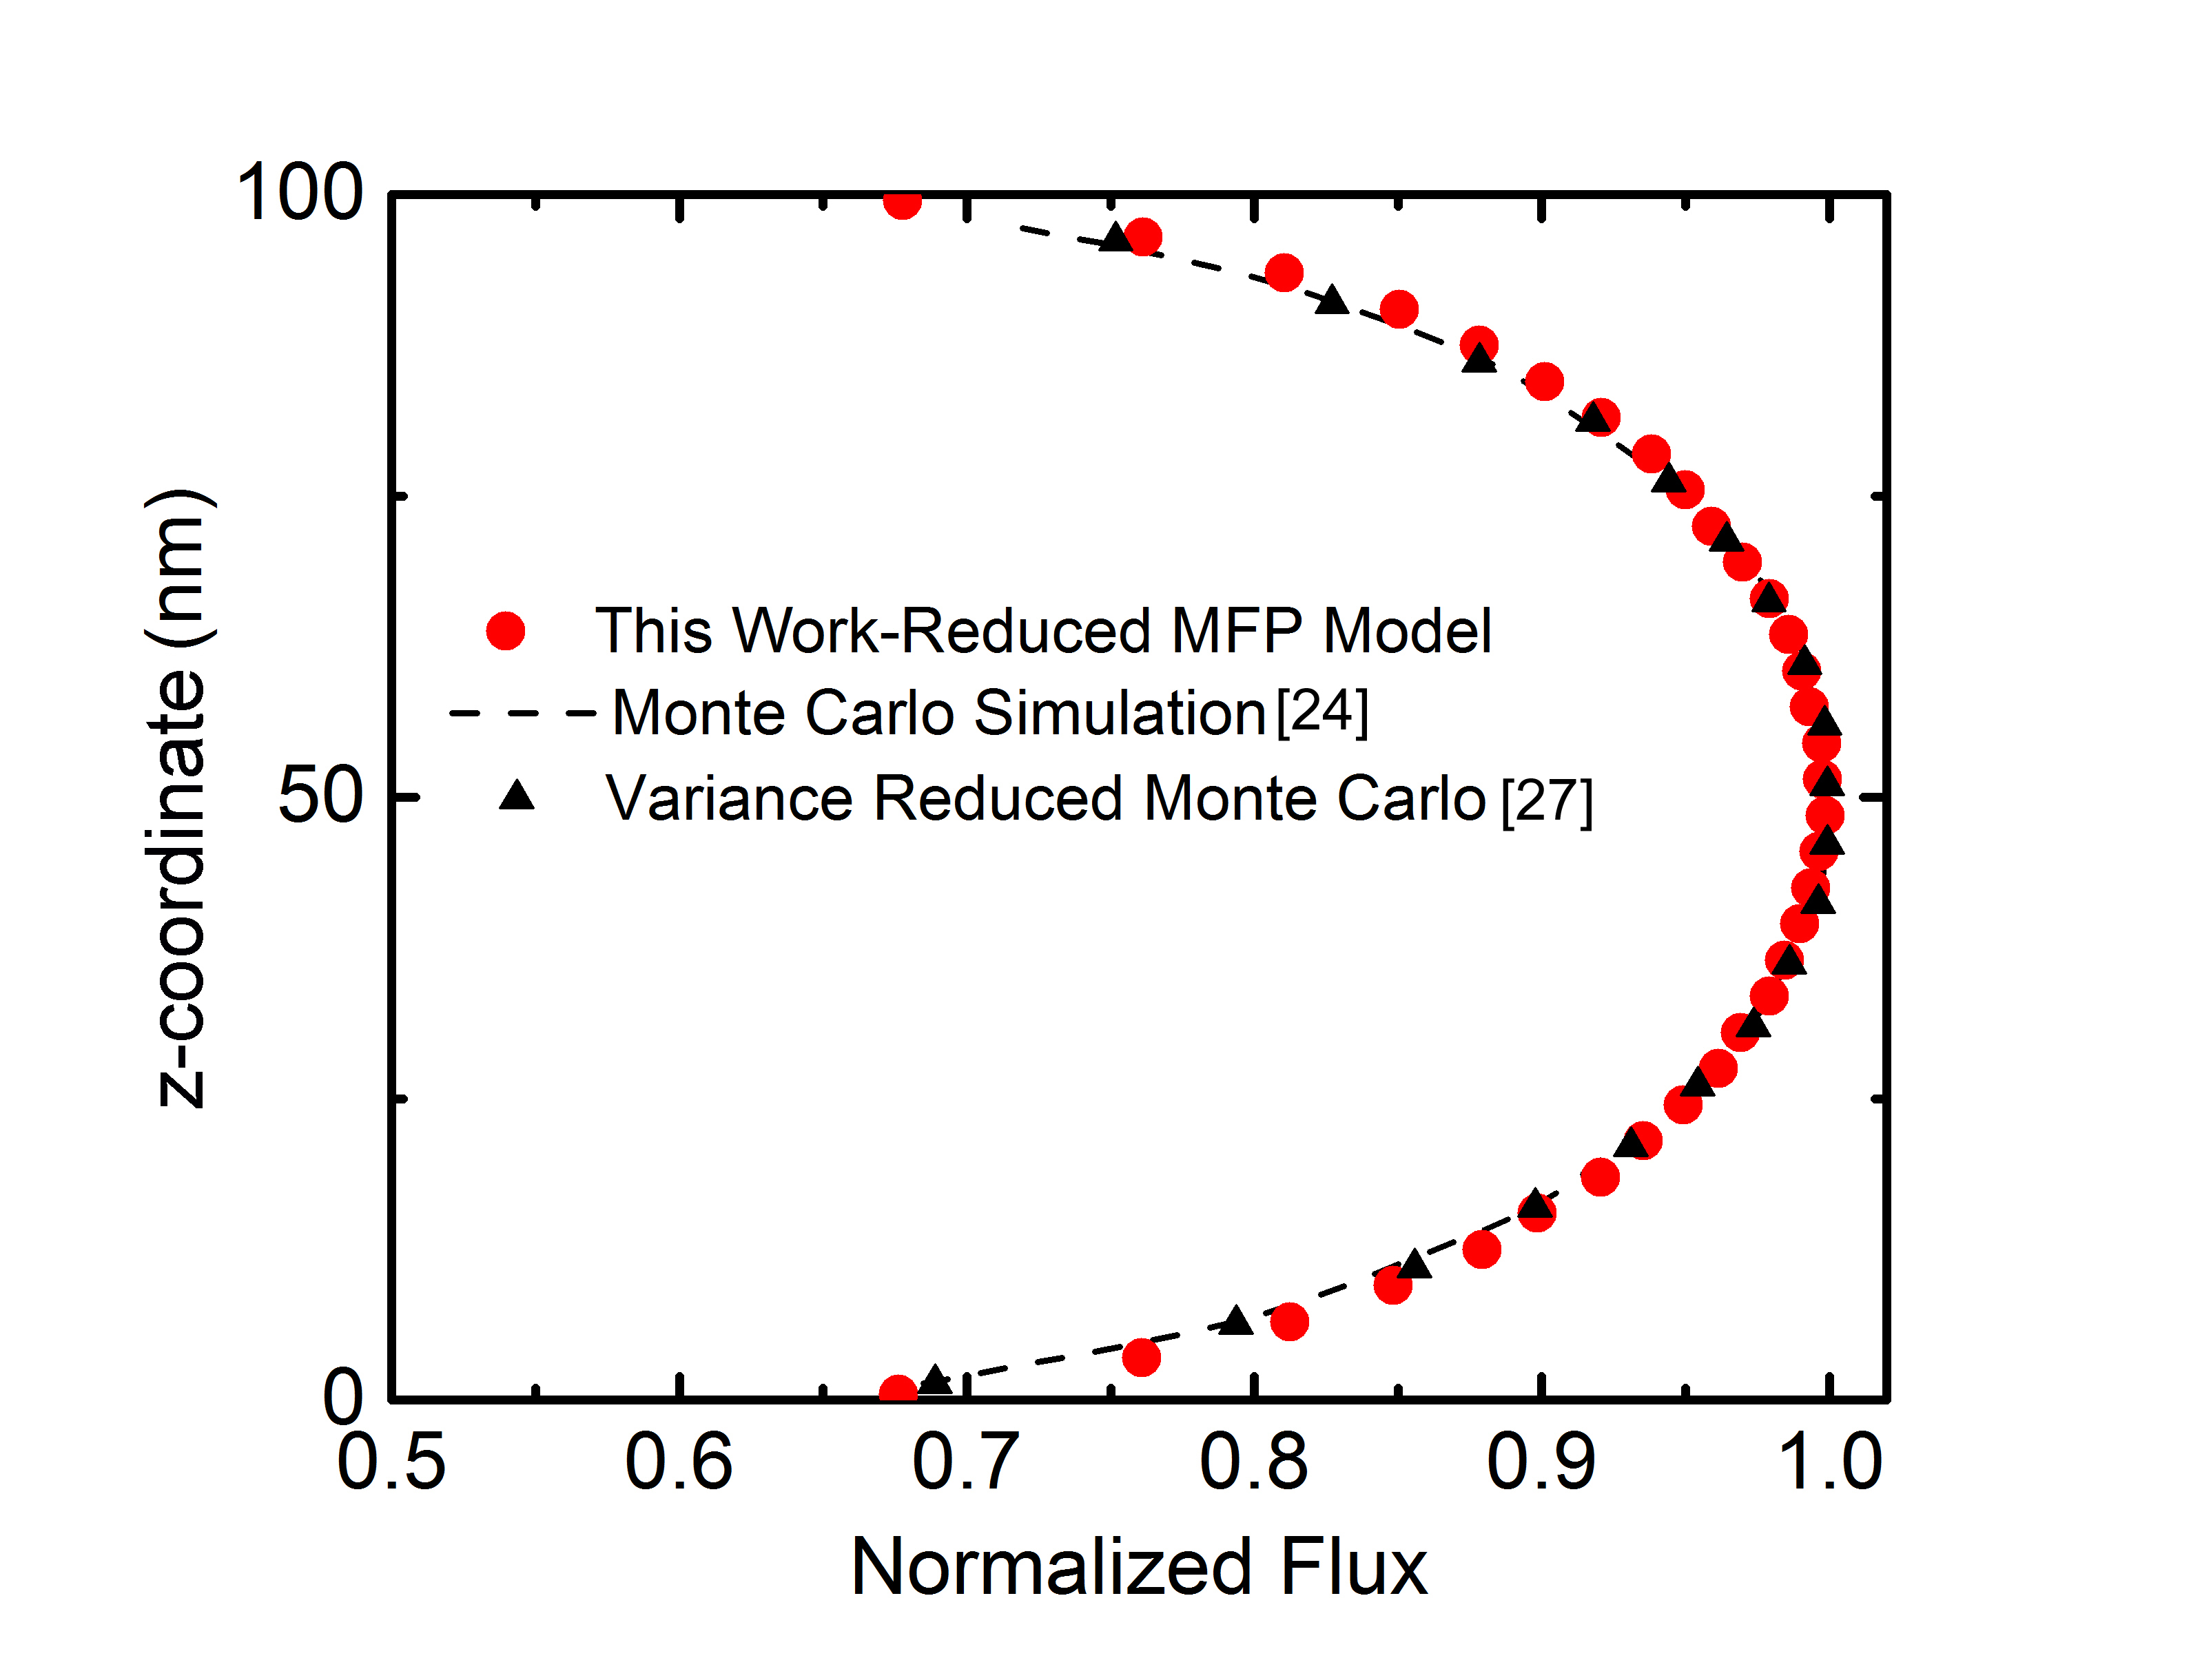
\includegraphics[width=0.95\textwidth]{/ch3/Fig3.jpg}
	\caption{Comparison of normalized heat flux in a 100nm Si thin film with fully diffusive upper and lower surfaces calculated by the reduced mean-free-path model (this work), Monte Carlo simulations \cite{RN445}, and variance-reduced Monte Carlo calculation \cite{RN276}. A maximum flux value is used for normalization.}
	\label{fig:ch3-comparison}
\end{figure}

Next, we use the flexibility of our reduced mean-free-path approach in terms of being able to treat general surface properties and study thermal transport properties and spatial distributions of thermal energy in thin films with surfaces possessing different roughnesses. We first analyze the effect of surface conditions on thermal flux distribution in a silicon thin film. We introduce a spatial asymmetry in the nanostructure by changing the surface properties of the boundaries of the thin film. Specifically, the roughness \gls{eta} (and correlation length \gls{cl}) for the upper surface is fixed to be $\eta^U$ = 4 nm ($\mathcal{L}^U = 10\eta^U$), and the surface properties of the lower surface are varied by changing the surface roughness to be $\eta^L$ = 0.25, 0.50, and 4.0 nm and maintaining the correlation length-to-roughness ratio ($\mathcal{L}^L = 10\eta^L$). In \Cref{fig:ch3-results-flux}, we show the existence of a thermal transport regime where heat conduction is spatially asymmetric, and the root of such a phenomenon lies in the differential behavior of the surface boundaries. As seen in the central panel of \Cref{fig:ch3-results-flux}, in a silicon film of thickness \gls{t} = 100 nm at room temperature, a roughness reduction at the lower surface (and corresponding correlation length) compared to the upper surface is accompanied by an increased asymmetry in the thermal flux, with more heat current flowing through the lower half of the film, as indicated by the increasing difference between the values of the thermal flux at the two boundaries. Additionally, the locus of peak flux shifts toward the lower surface as the difference in the roughness between the two boundaries is increased; that is, a larger proportion of thermal energy flows through the lower half of the thin film. Another key aspect of the flux profiles is the forward shift in the overall heat flux values corresponding to a net higher conduction in films with smoother surfaces. These results quantitatively show how an asymmetry in the surface properties of the two thin-film boundaries creates an asymmetry in the thermal flux within a thin film. \Cref{fig:ch3-results-flux}(a-c) show that the impact of distinct surface conditions on flux distributions is maintained across different thicknesses \gls{t} = 10, 100, 1000 nm. Note that the magnitude of flux increases overall with increasing thickness because the thermal transport at these length scales is quasi-ballistic and dependent on the size of the nanostructure. Importantly, the shape of the spatial flux diagram shows that, at an increased thickness [\Cref{fig:ch3-results-flux}(c)], the difference between the flux conducted near the edges of the thin film and at the center significantly increases. We also show in \Cref{fig:ch3-results-flux}(b,d,e) the impact of changes in temperature on the spatial distribution of thermal flux. A stronger role of the interfaces at lower temperatures is observed in the effective thermal flux due to the larger bulk phonon mean-free-paths. The changed magnitude of flux with temperature is also a consequence of modified internal scattering rates, with reduced phonon-phonon scattering rates occurring at lower temperatures. For the range of temperatures considered (\gls{T} = 100, 300, 700 K), the effects on the internal spatial distribution of the thermal energy is less pronounced than those arising from a change in the thickness of the film. Importantly, we have shown that heat flow can be manipulated to move closer to the center or near a surface of the film by purposely modifying the surface properties.
\par The observed behavior showing larger heat flux near smoother interfaces leads us to postulate that whereas a very rough diffuse boundary is analogous to fixed walls in fluid flow, a surface with small roughness (and in the limiting case of unity specularity) would be analogous to a plug fluid flow regime \cite{book_Bird}. We note that a surface boundary with specularity \gls{p} = 1 requires perfectly smooth thin-film boundaries devoid of any surface perturbations, which are difficult to create in experimentally grown Si nanostructures \cite{RN274,RN337}. \Cref{fig:ch3-results-flux-fluid}(a) shows normalized thermal flux profiles in thin films with limiting theoretical surface specularity values \gls{p} = 0 (completely diffuse) and \gls{p} = 1 (completely specular) for all phonons irrespective of their wavelength or incident angle. It is clearly seen that the heat flux near a diffusive boundary is suppressed, whereas phonon conduction near a specular boundary is less affected. Interestingly, when both surface boundaries are entirely specular, a constant thermal flux profile is obtained, analogous to a ``perfect plug flow" fluid velocity profile in a closed conduit. In this specular case, there is no randomization of phonon momentum upon encountering the surface, and the thermal flux is transported uninhibited. Such a constant thermal flux profile is also expected in bulk crystals. A nearly perfect plug flow is found in films with thicknesses in which the effects of the boundaries and interfacial phonon dynamics are negligible, as shown in the heat flux distribution calculated for a film of \gls{t} = 100 \si{\micro}m at room temperature [\Cref{fig:ch3-results-flux-fluid}(b)]. Most of the volume in a 100 \si{\micro}m silicon film is far away from the influence of the boundaries and exhibits a nearly constant, surface-independent flux similar to a perfect plug flow regime. Still the phonons close to the surfaces still interact with the boundaries (despite the overall dominating effect of internal phonon scattering processes in thicker films), creating their reduced mean-free-paths. %figure
\clearpage
\begin{sidewaysfigure}[hbt]
	\centering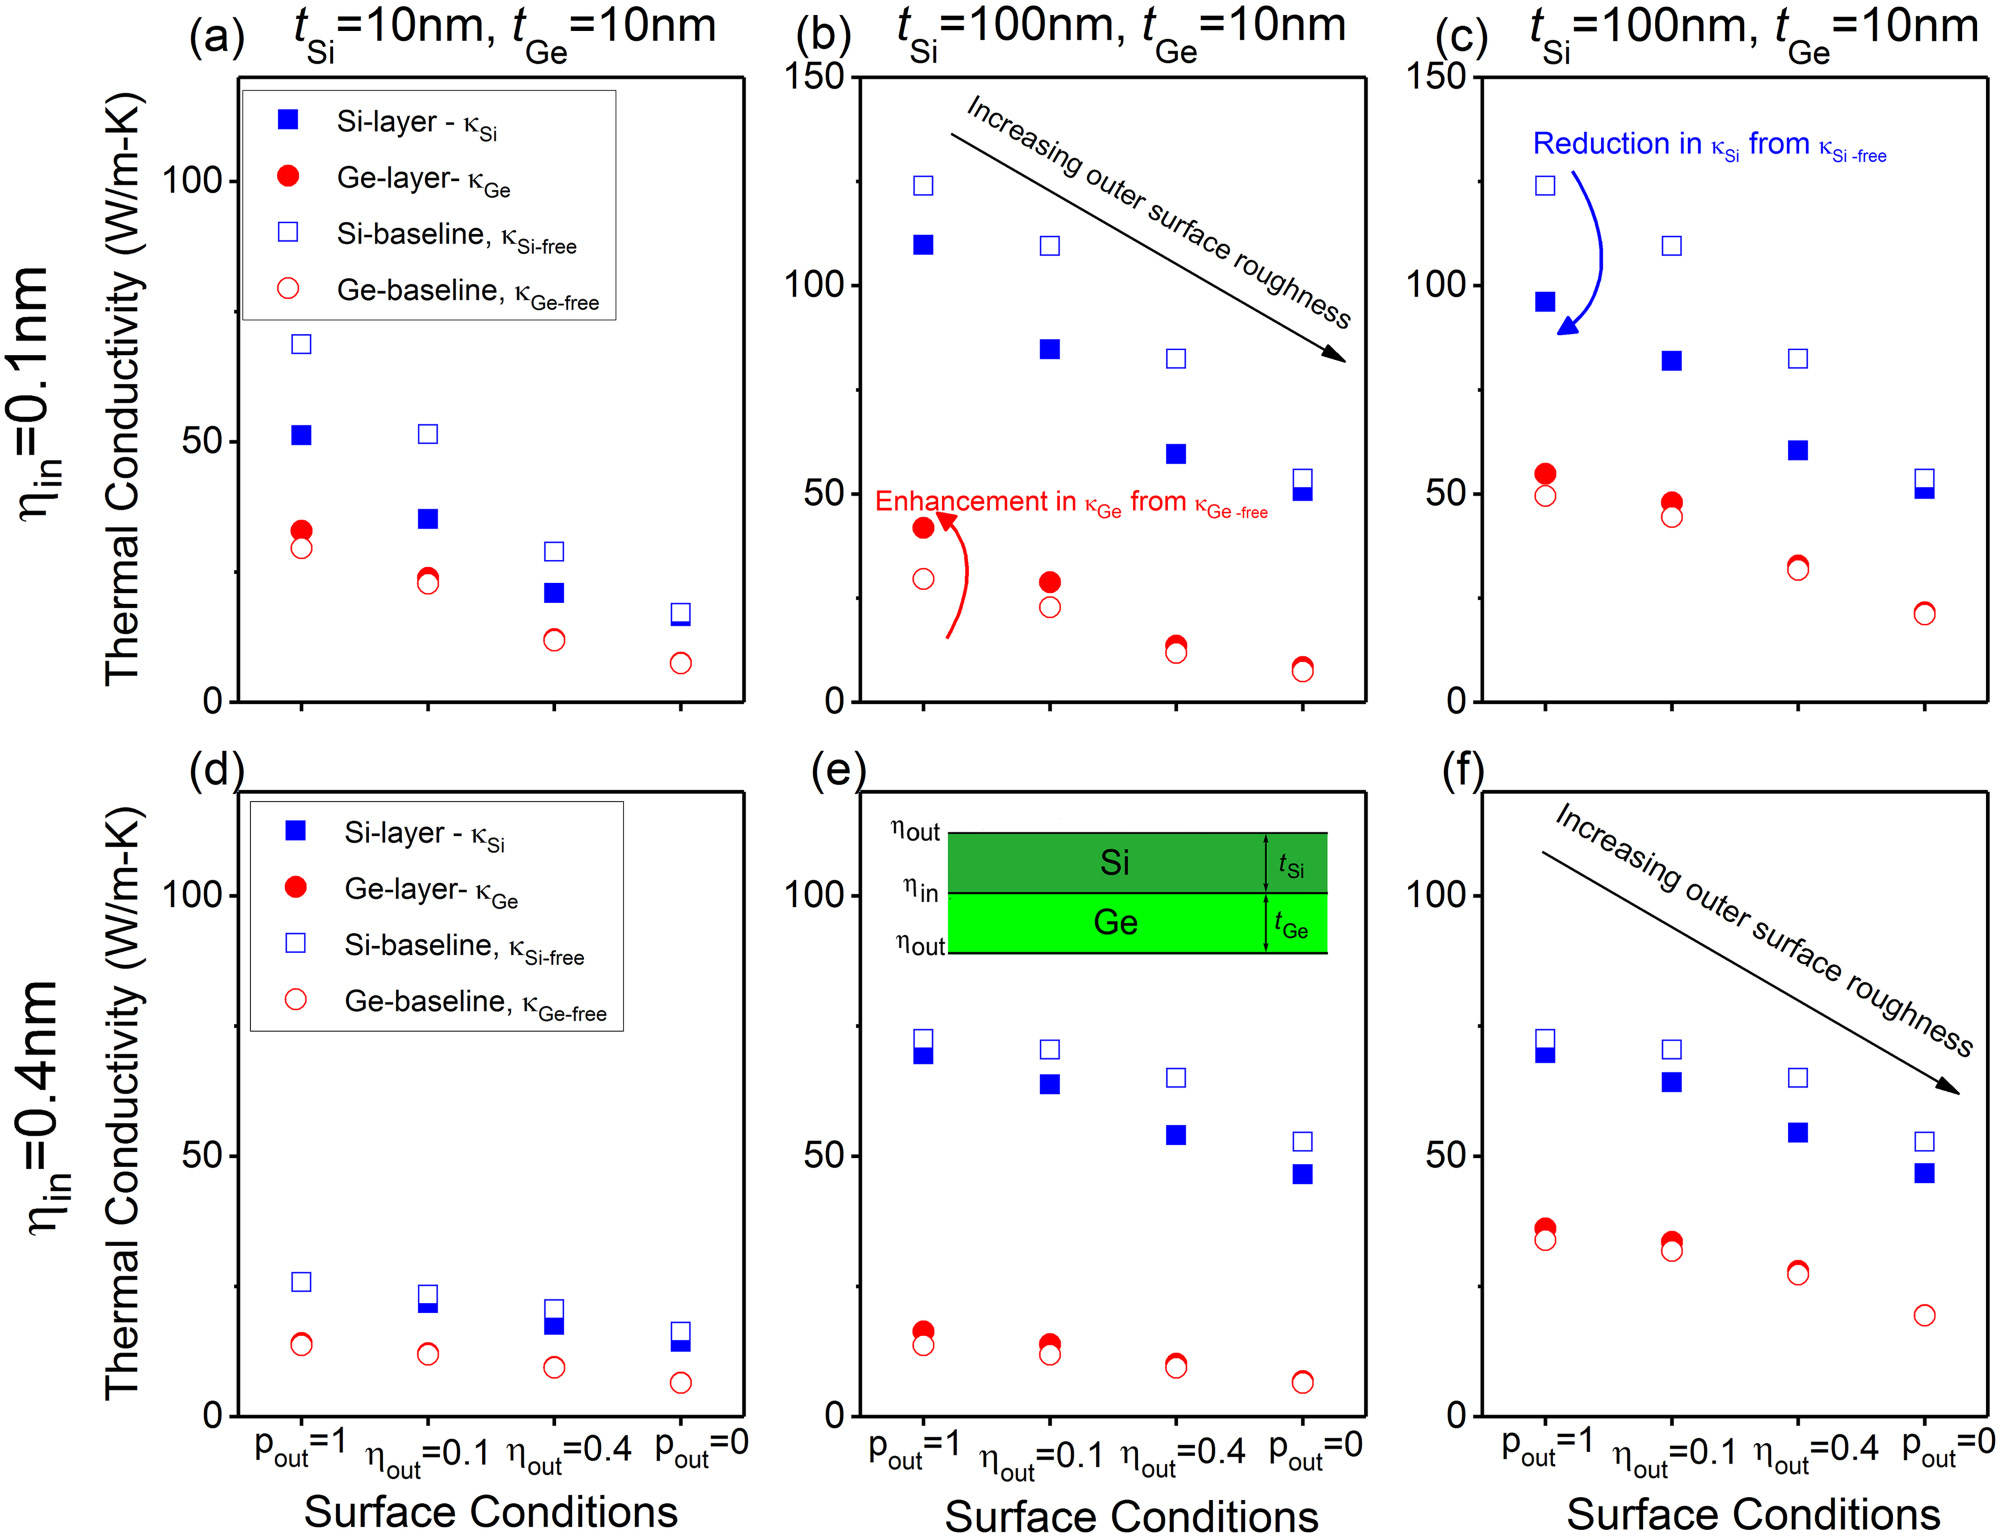
\includegraphics[width=1\textwidth]{/ch3/Fig4.jpg}
	\caption{Thermal flux profiles in Si thin films under a temperature gradient of 1\si{\kelvin\per\micro\meter} are shown as a function of temperature (\gls{T} = 100, 300, and 700 K) and thicknesses (\gls{t} = 10 nm, 100 nm, and 1 \si{\micro}m). Moving left to right, the thickness increases (upper panels) and the temperature decreases (lower panels). The central panel (b) shows the flux profiles at \gls{T} = 300 K and thickness \gls{t} = 100 nm. The surface roughness of the upper boundary is \gls{eta} = 4 nm and the roughness of the lower boundary is varied as \gls{eta} = 4 nm (blue), 0.5 nm (green), and 0.25 nm (red lines). The correlation length \gls{cl} is 10 times the roughness at both the surfaces.}
	\label{fig:ch3-results-flux}
\end{sidewaysfigure}
\clearpage
%figure
\begin{figure}[hbt]
	\centering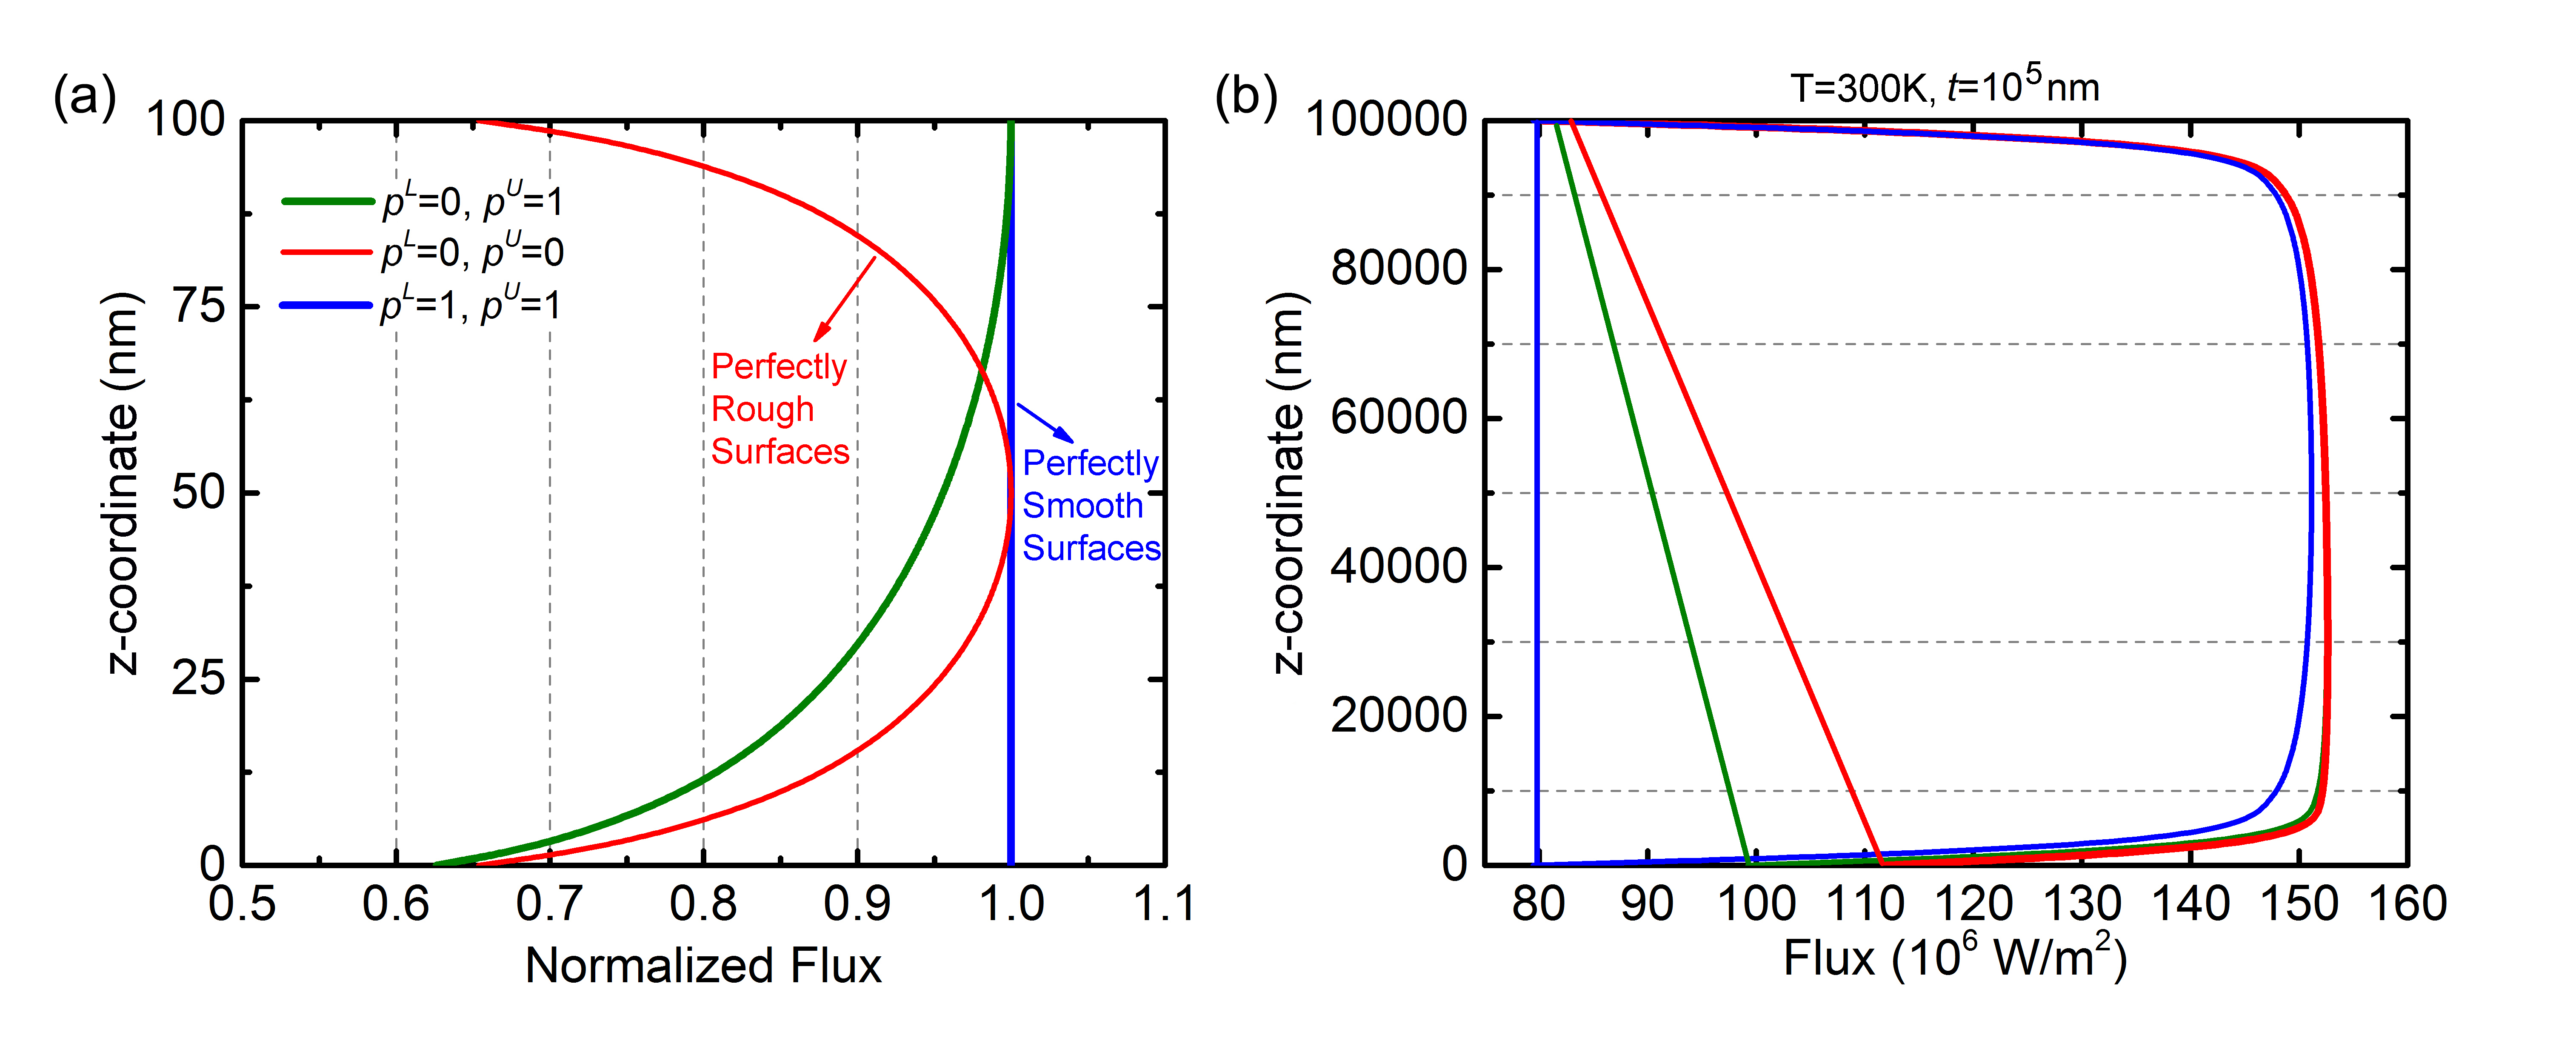
\includegraphics[width=1\textwidth]{/ch3/Fig5.jpg}
	\caption{(a) Normalized thermal flux profiles in an Si thin film with varying surface conditions (limiting cases \gls{p} = 0 and \gls{p} = 1) are shown for a film thickness of \gls{t} = 100 nm at room temperature. (b) Nearly ideal plug flow profile development in very thick films where variations in thermal flux spatial distribution is constrained around the boundaries.}
	\label{fig:ch3-results-flux-fluid}
\end{figure}

Thus, the thermal flux deviates significantly from the bulk value only at spatial locations in the vicinity of the thin-film boundaries. However, because this deviation occurs in a very small spatial domain (compared to the overall thickness of the film), the averaged thermal conductivity is nearly unaffected by the deviations from plug flow flux profile in such large thickness films.
\section{Summary}
In this chapter, we analyzed the most general case of thin films; i.e., films with boundaries possessing independent surface properties. To study heat conduction processes in such thin-films, we developed two approaches. The first approach is based on determining the reduced phonon mean-free-path while the second approach is based on solving BTE to obtain non-equilibrium phonon populations. After establishing their equivalence, the former approach was utilized to evaluate thermal fluxes. We found that heat flux can be engineered to flow close to a surface or near the center of the film. We also showed the existence of heat transport regimes resembling fluid flow in confined geometries. The development of asymmetry in thermal flux with increasing difference between interface roughness properties were established. The results in this chapter show that computational tools with accurate boundary scattering mechanisms can yield insights about thermal transport phenomena and underscore the importance of interfacial phonon dynamics in heat conduction pathways in nanostructures. Furthermore, the methods described here move beyond the commonly used diffuse scattering surface assumptions, enabling the surfaces of nanostructures to be precisely described, strengthening the predictive power of models.
